\documentclass[]{article}
\voffset=-1.5cm
\oddsidemargin=0.0cm
\textwidth = 470pt


\usepackage{amsmath}
\usepackage{graphicx}
\usepackage{amssymb}
\usepackage{framed}
% % - http://statweb.stanford.edu/~susan/courses/s141/exanova.pdf
\begin{document}
	
	\large
	\tableofcontents
	\newpage
	%----------------------------------------------%
\newpage

\begin{center}
{\fontsize{2.5cm}{1em}\selectfont \[ \sum \]}
{\fontsize{1.5cm}{1em}\selectfont\textbf{ Discrete Mathematics} }\\ \bigskip
{\fontsize{0.8cm}{1em}\textrm{Mathematics for Computing}}\\
\end{center}
\newpage

\section{TWO-WAY ANALYSIS OF VARIANCE (TWO-WAY ANOVA)}
\begin{framed}
\noindent The two-way ANOVA compares the mean differences between groups that have been split on two independent variables (called factors). 

The primary purpose of a two-way ANOVA is to understand if there is an interaction between the two independent variables on the dependent variable.
\end{framed}


Use two-way anova when you have one measurement variable and two nominal variables, and each value of one nominal variable is found in combination with each value of the other nominal variable.


\begin{itemize}
\item Two-way analysis of variance is based on two dimensions of classifications, or treatments. For example, in
analyzing the level of achievement in a training program we could consider both the effect of the method of
instruction and the effect of prior school achievement. \item Similarly, we could investigate gasoline mileage
according to the weight category of the car and according to the grade of gasoline. 
\item In data tables, the treatments
identified in the column headings are typically called the \textbf{\textit{A treatments}}; those in the row headings are called the \textbf{\textit{B
treatments}}.
\end{itemize}

\subsection{Laerd}
Two-way ANOVA in SPSS Statistics

Introduction
The two-way ANOVA compares the mean differences between groups that have been split on two independent variables (called factors). The primary purpose of a two-way ANOVA is to understand if there is an interaction between the two independent variables on the dependent variable. For example, you could use a two-way ANOVA to understand whether there is an interaction between gender and educational level on test anxiety amongst university students, where gender (males/females) and education level (undergraduate/postgraduate) are your independent variables, and test anxiety is your dependent variable. Alternately, you may want to determine whether there is an interaction between physical activity level and gender on blood cholesterol concentration in children, where physical activity (low/moderate/high) and gender (male/female) are your independent variables, and cholesterol concentration is your dependent variable.

The interaction term in a two-way ANOVA informs you whether the effect of one of your independent variables on the dependent variable is the same for all values of your other independent variable (and vice versa). For example, is the effect of gender (male/female) on test anxiety influenced by educational level (undergraduate/postgraduate)? Additionally, if a statistically significant interaction is found, you need to determine whether there are any "simple main effects", and if there are, what these effects are (we discuss this later in our guide).

Note: If you have three independent variables rather than two, you need a three-way ANOVA.

%In this "quick start" guide, we show you how to carry out a two-way ANOVA using SPSS Statistics, as well as interpret and report the results from this test. However, before we introduce you to this procedure, you need to understand the different assumptions that your data must meet in order for a two-way ANOVA to give you a valid result. We discuss these assumptions next.
%====================================================================================================================%
\section{Assumptions}
\begin{itemize}
\item The populations from which the samples were obtained must be normally or approximately normally distributed.
\item The samples must be independent.
\item The variances of the populations must be equal.
\item The groups must have the same sample size.
\end{itemize}
\subsection{LAERD}



When you choose to analyse your data using a two-way ANOVA, part of the process involves checking to make sure that the data you want to analyse can actually be analysed using a two-way ANOVA. You need to do this because it is only appropriate to use a two-way ANOVA if your data "passes" six Assumptions that are required for a two-way ANOVA to give you a valid result. In practice, checking for these six Assumptions means that you have a few more procedures to run through in SPSS Statistics when performing your analysis, as well as spend a little bit more time thinking about your data, but it is not a difficult task.

Before we introduce you to these six Assumptions, do not be surprised if, when analysing your own data using SPSS Statistics, one or more of these Assumptions is violated (i.e., is not met). This is not uncommon when working with real-world data rather than textbook examples, which often only show you how to carry out a two-way ANOVA when everything goes well! However, don’t worry. Even when your data fails certain Assumptions, there is often a solution to overcome this. First, let’s take a look at these six Assumptions:
\begin{description}
\item[ Assumption 1:] Your dependent variable should be measured at the continuous level (i.e., they are interval or ratio variables). Examples of continuous variables include revision time (measured in hours), intelligence (measured using IQ score), exam performance (measured from 0 to 100), weight (measured in kg), and so forth. You can learn more about interval and ratio variables in our article:] Types of Variable.
\item[ Assumption 2:] Your two independent variables should each consist of two or more categorical, independent groups. Example independent variables that meet this criterion include gender (2 groups:] male or female), ethnicity (3 groups:] Caucasian, African American and Hispanic), profession (5 groups:] surgeon, doctor, nurse, dentist, therapist), and so forth.
\item[ Assumption 3:] You should have independence of observations, which means that there is no relationship between the observations in each group or between the groups themselves. For example, there must be different participants in each group with no participant being in more than one group. This is more of a study design issue than something you would test for, but it is an important Assumption of the two-way ANOVA. If your study fails this Assumption, you will need to use another statistical test instead of the two-way ANOVA (e.g., a repeated measures design). If you are unsure whether your study meets this Assumption, you can use our Statistical Test Selector, which is part of our enhanced guides.
\item[ Assumption 4:] There should be no significant outliers. Outliers are data points within your data that do not follow the usual pattern (e.g., in a study of 100 students' IQ scores, where the mean score was 108 with only a small variation between students, one student had a score of 156, which is very unusual, and may even put her in the top 1% of IQ scores globally). The problem with outliers is that they can have a negative effect on the two-way ANOVA, reducing the accuracy of your results. Fortunately, when using SPSS Statistics to run a two-way ANOVA on your data, you can easily detect possible outliers. In our enhanced two-way ANOVA guide, we:] (a) show you how to detect outliers using SPSS Statistics; and (b) discuss some of the options you have in order to deal with outliers.
\item[ Assumption 5:] Your dependent variable should be approximately normally distributed for each combination of the groups of the two independent variables. Whilst this sounds a little tricky, it is easily tested for using SPSS Statistics. Also, when we talk about the two-way ANOVA only requiring approximately normal data, this is because it is quite "robust" to violations of normality, meaning the Assumption can be a little violated and still provide valid results. You can test for normality using the Shapiro-Wilk test for normality, which is easily tested for using SPSS Statistics. In addition to showing you how to do this in our enhanced two-way ANOVA guide, we also explain what you can do if your data fails this Assumption (i.e., if it fails it more than a little bit).
\item[ Assumption 6:] There needs to be homogeneity of variances for each combination of the groups of the two independent variables. Again, whilst this sounds a little tricky, you can easily test this Assumption in SPSS Statistics using Levene’s test for homogeneity of variances. In our enhanced two-way ANOVA guide, we (a) show you how to perform Levene’s test for homogeneity of variances in SPSS Statistics, (b) explain some of the things you will need to consider when interpreting your data, and (c) present possible ways to continue with your analysis if your data fails to meet this Assumption.
\end{description}
You can check Assumptions 4, 5 and 6 using SPSS Statistics. Before doing this, you should make sure that your data meets Assumptions 1, 2 and 3, although you don’t need SPSS Statistics to do this. Just remember that if you do not run the statistical tests on these Assumptions correctly, the results you get when running a two-way ANOVA might not be valid. This is why we dedicate a number of sections of our enhanced two-way ANOVA guide to help you get this right. You can find out about our enhanced content as a whole here, or more specifically, learn how we help with testing Assumptions here.

In the section, Test Procedure in SPSS Statistics, we illustrate the SPSS Statistics procedure to perform a two-way ANOVA Assuming that no Assumptions have been violated. 

First, we set out the example we use to explain the two-way ANOVA procedure in SPSS Statistics.

\section{Hypotheses}

There are three sets of hypothesis with the two-way ANOVA. The null hypotheses for each of the sets are given below.

\begin{itemize}
\item The population means of the first factor are equal. \\ \textit{This is like the one-way ANOVA for the row factor.}
\item The population means of the second factor are equal. \textit{This is like the one-way ANOVA for the column factor.}
\item There is no interaction between the two factors. \textit{This is similar to performing a test for independence with contingency tables}.
\end{itemize}

\section{Factors}

The two independent variables in a two-way ANOVA are called factors. The idea is that there are two variables, factors, which affect the dependent variable. Each factor will have two or more levels within it, and the degrees of freedom for each factor is one less than the number of levels.

\section{Main Effect}

\begin{itemize}
\item The main effect involves the independent variables separately. 
\item The interaction is ignored for this part. Just the rows or just the columns are used, not mixed. 
\item This is the part which is similar to the one-way analysis of variance. 
\item Each of the variances calculated to analyze the main effects are like the between variances
\end{itemize}



\section{Treatment Groups}
\begin{itemize}
	\item Treatement Groups are formed by making all possible combinations of the two factors. 
	\item For example, if the first factor has 3 levels and the second factor has 2 levels, then there will be $3\times 2=6$ different treatment groups.
	\item There may be more than one observation per treatment group.
\end{itemize}

\section{Interaction Effect}
\begin{itemize}
\item The interaction effect is the effect that one factor has on the other factor. 
\item The degrees of freedom here is the product of the two degrees of freedom for each factor. 
\item \textbf{Important:} The interaction effect can only be computed in the case of multiple measurements per treatment group.
\end{itemize}


\section{Within Variation}
\begin{itemize}
	\item The \textbf{\textit{Within variation}} is the sum of squares within each treatment group. 
	\item You have one less than the sample size (remember all treatment groups must have the same sample size for a two-way ANOVA) for each treatment group. 
	\item The total number of treatment groups is the product of the number of levels for each factor. 
	\item The within variance is the within variation divided by its degrees of freedom.
\end{itemize}


%The within group is also called the error.


\subsection{Corn Example}
\begin{itemize}
\item As an example, let's assume we're planting corn. The type of seed and type of fertilizer are the two factors we're considering in this example. This example has 15 treatment groups. 
\item There are 3-1=2 degrees of freedom for the type of seed, and 5-1=4 degrees of freedom for the type of fertilizer. 
\item There are $2\times4 = 8$ degrees of freedom for the interaction between the type of seed and type of fertilizer.
\end{itemize}


The data that actually appears in the table are samples. In this case, 2 samples from each treatment group were taken.

\begin{tabular}{|c|c|c|c|c|c|}
	\hline  & Fert I &	Fert II	&Fert III &	Fert IV	& Fert V \\ \hline
	Seed A-402 &	106, 110 &	95, 100	& 94, 107 &	103, 104 &	100, 102 \\ \hline
	Seed B-894&	110, 112 &	98, 99&	100, 101&	108, 112&	105, 107 \\ \hline
	Seed C-952&	94, 97	& 86, 87&	98, 99&	99, 101&	94, 98 \\ \hline
\end{tabular} 


\section{F-Tests}

There is an F-test for each of the hypotheses, and the F-test is the mean square for each main effect and the interaction effect divided by the within variance. The numerator degrees of freedom come from each effect, and the denominator degrees of freedom is the degrees of freedom for the within variance in each case.

\section{Two-Way ANOVA Table}

\begin{itemize}
\item It is assumed that main effect A has a levels (and A = a-1 df), main effect B has b levels (and B = b-1 df), n is the sample size of each treatment, and N = abn is the total sample size. \item Notice the overall degrees of freedom is once again one less than the total sample size.
\end{itemize}

\begin{figure}
\centering
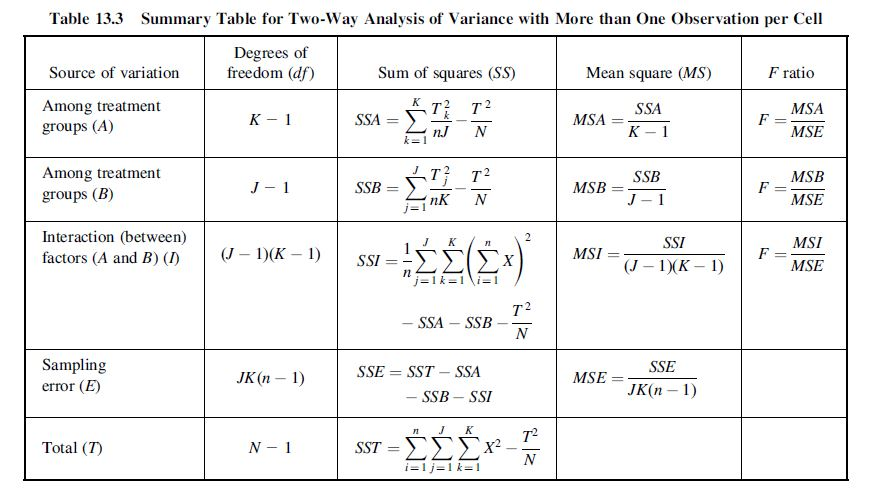
\includegraphics[width=1.1\linewidth]{TwoWayANOVA-Table2}
\caption{}
\label{fig:TwoWayANOVA-Table2}
\end{figure}
 
%==================================================================================== %

\[ \textrm{MS}_{Trt} = c \times S^2_{R}\]
\[ \textrm{MS}_{Block} = r \times S^2_{C}\]

\begin{itemize}
	\item $r$ and $c$ are the numbers of rows and columns respectively.
	\item $S^2_{R}$ is the variance of the Row means 
	\item $S^2_{C}$ is the variance of the column means.
\end{itemize}

Take care when working with calculations that involve $r$ and $c$: 
$r$ is the number of rows, which is the number of subgroups for each of the treatments (which are arranged along the columns).
$c$ is the number of columns, which is the number of subgroups for each of the blocks (which are arranged along the rows).

%===========================================================================%
\newpage
\section{Worked Example}

Three varieties of potatoes are being compared for yield. The experiment
was carried out by assigning each variety at random to four of twelve equal size
plots, one being chosen in each of four locations. The following yields in bushels7 per 7
plot resulted:
A bushel is about 36.4 litres.

\begin{figure}[h!]
\centering
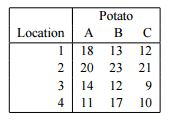
\includegraphics[width=0.4\linewidth]{twowayanova-potato}
\end{figure}
\subsection*{Additional Information} 
\begin{framed}
\noindent Expect to be given $S^2_R$ and $S^2_C$ in an exam standard question, as well as the variance for the response variable. You will also be given the formula for $\textrm{MS}_{Trt}$ and $\textrm{MS}_{Block}$.
\end{framed}
\begin{itemize}
\item The variance of the Row means is : $S^2_{R} = 19.037$. Therefore 
	\[ \textrm{MS}_{Trt} = c \times S^2_{R} = 3 \times 19.037 = 57.111 \]
	
\item the variance of the Column means is : $S^2_{C} = 3.0625$.	Therefore 
	\[ \textrm{MS}_{Block} = r \times S^2_{C} = 4 \times 3.0625 = 12.25\]
	
\item Also the overall variance of the 12 observations is \[\textrm{Var}(Y) = 21.6363 \]. 
\end{itemize}
\newpage
\subsection{Solution}

\begin{itemize}
	\item Here the treatment is \textbf{\textit{Location}}
	\item The block variable is \textbf{\textit{Type of Potato}}
\end{itemize}

\noindent \textbf{Step 1 :} We have already be given information that we can incorporate into our solution, once we have done the necessary calculations.

\bigskip
\noindent \textit{(Remark: The following calculation for $SS_{Tot}$ features in each ANOVA procedures on the course).}
\[\textrm{Var}(Y) = \frac{ SS_{tot}}{n-1} \]
\[ 21.6363 = \frac{ SS_{tot}}{12-1} \]
\[ SS_{tot} = 21.6362 \times 11 = 238 \]
{
	\Large
	\begin{center}
\begin{tabular}{|c|c|c|c|c|c|}
\hline Source	       &	df	&	SS	&	MS	&	F	&	p.values	\\ \hline
Treatment      &		&		&	57.111	&		&		\\ \hline
Block	&		\phantom{spa}		&	\phantom{spa}		&	12.25	&		&		\\ \hline
Total	&		&		&		\phantom{spa}		&	\phantom{spa}		&		\\ \hline 
Total	&	11	&	238	&		&		&		\\ \hline  
\end{tabular}
\end{center}
}

\bigskip

\noindent \textbf{Step 2 :} We will now determine the Degrees of Freedom for Blocks, Treatments and Error.

\begin{itemize}
	\item There are 4 types of treatment. The degrees of freedom for treament is therefore 3 ($r-1$).
	\item There are 3 blocks. The degrees of freedom for blocks is therefore 2 (i.e. $c-1$). 
	\item The total degrees of freedom should add up to 11. Therefore the degrees of freedom for error is 6.
	(i.e. $(r-1)\times (c-1)$. )
	\item \textbf{Remark:} Do not confuse $r-1$ with $c$. Here both are equal to 3, but this is a co-incidence.
\end{itemize}

{
	\Large
	\begin{center}
\begin{tabular}{|c|c|c|c|c|c|}
\hline Source	       &	df	&	SS	&	MS	&	F	&	p.values	\\ \hline
Treatment      &	3	&		&	57.111	& \phantom{spa} \phantom{spa}		&	\phantom{spa}	\\ \hline
Block	&	2	&		&	12.25	&		&		\\ \hline
Error	&	6	&	\phantom{spa}	&		&		&		\\ \hline 
Total	&	11	&	238	&		&		&		\\ \hline 
\end{tabular}
\end{center}
}


\newpage


\noindent \textbf{Step 3 :} In general, Mean Square Terms are computed by dividing the relevant SS terms by the corresponding degrees of freedom.

\[ MS = \frac{SS}{df} \]

\noindent Rearranging this , we can say : $SS = MS \times df$. Therefore

\begin{itemize}
	\item SS$_{Trt}$ = $3 \times 57.111 = 171.33 $
	\item SS$_{Block}$ = $2 \times 12.25 = 24.50$
\end{itemize}

Importantly 
\begin{framed}
	\[ SS_{tot} = SS_{trt} + SS_{block} +  SS_{error}\]
\end{framed}
We can compute $SS_{error}$
\[ 238 = 171.33 + 24.5 + SS_{error} \]

Necessarily $SS_{error} = 42.166$

{
\Large
\begin{center}
\begin{tabular}{|c|c|c|c|c|c|}
\hline Source	       &	df	&	SS	&	MS	&	F	&	p.values	\\ \hline
Treatment      &	3	&	171.333	&	57.111	&		&		\\ \hline
Block	&	2	&	24.50	&	12.25	&		&		\\ \hline
Error	&	6	&	42.166	&		\phantom{spa}		&	\phantom{spa}	&		\\ \hline 
Total	&	11	&	238	&		&		&		\\ \hline 
\end{tabular}
\end{center}
}

\newpage


\noindent \textbf{Step 4 :} We can now complete the table as follows
\begin{itemize}
	\item $MS_{error}$
	
	\[ MS_{error} = \frac{SS_{error}}{df_{error}} - \frac{42.166}{6} = 7.033\]
	
	\item Test Statistic 1
	\[F_{Trt} = \frac{MS_{Trt}}{ MS_error } = \frac{57.111}{7.033} = 8.12 \]
	
	\item Test Statistic 1
	\[F_{Block} = \frac{MS_{Block}}{ MS_error } = \frac{12.15}{7.033} = 1.74 \]
\end{itemize}

%=================================================================%
{
	\Large
	\begin{center}
		\begin{tabular}{|c|c|c|c|c|c|}
\hline Source	       &	df	&	SS	&	MS	&	F	&	p.values	\\ \hline
Treatment      &	3	&	171.333	&	57.111	&	8.12	&		\\ \hline
Block	&	2	&	24.50	&	12.250	&	1.74	&		\\ \hline
Error	&	6	&	42.166	&	7.033	&		&		\\ \hline 
Total	&	11	&	238	&		&\phantom{spa}		&	\phantom{spa}		\\ \hline 
\end{tabular}
\end{center}
}


\newpage
%============================================================================== %
\section{Summary}

The following results are calculated using the Quattro Pro spreadsheet. It provides the p-value and the critical values are for alpha = 0.05.
\begin{figure}
\centering
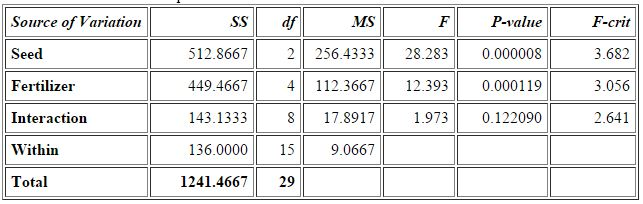
\includegraphics[width=0.7\linewidth]{QuattroPro}
\caption{}
\label{fig:QuattroPro}
\end{figure}
 	 	 
From the above results, we can see that the main effects are both significant, but the interaction between them isn't. That is, the types of seed aren't all equal, and the types of fertilizer aren't all equal, but the type of seed doesn't interact with the type of fertilizer.



\section{Interaction}
\begin{itemize}
\item Interaction in a two-factor experiment means that the two treatments are not independent, and that the
effect of a particular treatment in one factor differs according to levels of the other factor. 
\item For example, in
studying automobile mileage a higher-octane gasoline may improve mileage for certain types of cars but not for
others. Similarly, the effectiveness of various methods of instruction may differ according to the ability levels of
the students. 
\item In order to test for interaction, more than one observation or sampled measurement (i.e.,
replication) has to be included in each cell of the two-way data table. 
\item Section 13.4 presents the analytical
procedure that is appropriate when there is only one observation per cell, and in which interaction between the
two factors cannot be tested. 
\item The analytical procedure is extended to include replication and the analysis of
interaction effects in Section 13.5.
\end{itemize}

%======================================================================================================================%
\newpage
\section{13.4 THE RANDOMIZED BLOCK DESIGN}
\noindent \textbf{(TWO-WAY ANOVA, ONE OBSERVATION PER CELL)}
\begin{itemize}
\item The two-way analysis of variance model in which there is only one observation per cell is generally
referred to as the randomized block design, because of the principal use for this model. What if we extend the
idea of using paired observations to compare two sample means (see Section 11.3) to the basic one-way analysis
of variance model, and have groups of k matched individuals assigned randomly to each treatment level? In
analysis of variance, such matched groups are called blocks, and because the individuals (or items) are
randomly assigned based on the identified block membership, the design is referred to as the randomized block
design. 
\item In such a design the blocks dimension is not a treatment dimension as such. The objective of using this
design is not for the specific purpose of testing for a blocks effect. Rather, by being able to assign some of the
variability among subjects to prior achievement, for example, the MSE can be reduced and the resulting test of
the A treatments effect is more sensitive.
\end{itemize}

%======================================================================================================================%
Summary Table for One-Way Analysis of Variance (Treatment Groups Need Not Be Equal)
Source of variation
Degrees of freedom
(df )
Sum of squares
(SS)

The linear model for the two-way analysis of variance model with one observation per cell (with no
replication) is

\begin{figure}
\centering
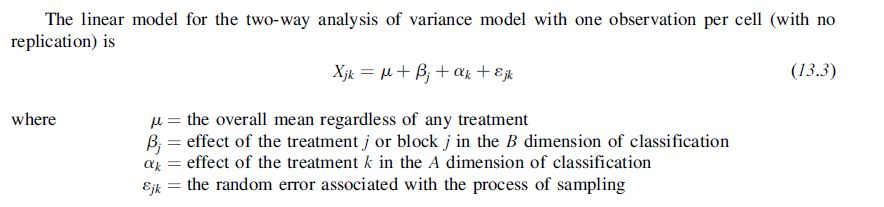
\includegraphics[width=1.1\linewidth]{TwoWayANOVA-Equation1}
\end{figure}

Table 13.2 is the summary table for the two-way analysis of variance without replication. As compared
with Table 13.1 for the one-way analysis of variance, the only new symbol in this table is T2
j , which indicates
that the total of each j group (for the B treatments, or blocks) is squared. See Problems 13.5 and 13.6 for
application of these formulas.
%================================================================================================ %
\section{13.5 TWO-FACTOR COMPLETELY RANDOMIZED DESIGN}
\noindent \textbf{(TWO-WAY ANOVA, n OBSERVATIONS PER CELL)}

\begin{itemize}
\item As explained in Section 13.3, when replication is included within a two-way design, the interaction
between the two factors can be tested.
\item Thus, when such a design is used, three different null hypotheses can be
tested by the analysis of variance: that there are no column effects (the column means are not significantly
different), that there are no row effects (the row means are not significantly different), and that there is no
interaction between the two factors (the two factors are independent). 
\item A significant interaction effect indicates
that the effect of treatments for one factor varies according to levels of the other factor. 
\item In such a case, the
existence of column and/or row effects may not be meaningful from the standpoint of the application of
research results.
\end{itemize}
%======================================================================================================================%
The linear model for the two-way analysis of variance when replication is included is
\begin{figure}
\centering
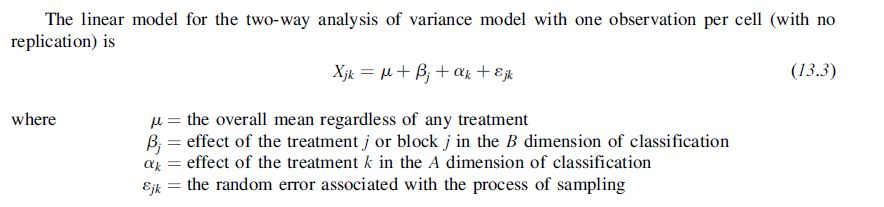
\includegraphics[width=1.1\linewidth]{TwoWayANOVA-Equation1}
\caption{}
\label{fig:TwoWayANOVA-Equation1}
\end{figure}

Table 13.2 Summary Table for Two-Way Analysis of Variance with One Observation per Cell (Randomized
Block Design)
\begin{figure}
\centering
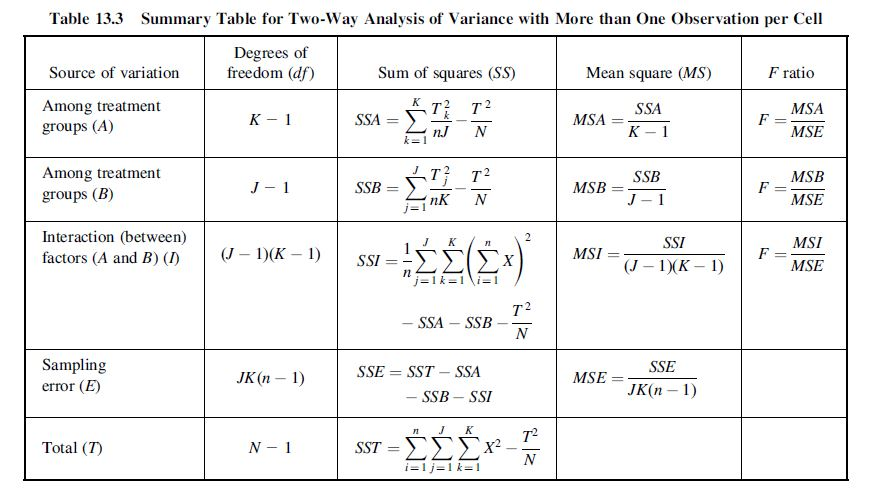
\includegraphics[width=0.7\linewidth]{TwoWayANOVA-Table2}
\caption{}
\label{fig:TwoWayANOVA-Table2}
\end{figure}


%======================================================================================================================%
Table 13.3 is the summary table for the two-way analysis of variance with replication. The formulas
included in this table are based on the assumption that there are an equal number of observations in all of the
cells. See Problem 13.7 for application of these formulas.
%======================================================================================================================%
\newpage
\section{13.6 ADDITIONAL CONSIDERATIONS}
\begin{itemize}
\item All of the computational procedures presented in this chapter are for fixed-effects models of the analysis of
variance. 
\item In a fixed-effects model, all of the treatments of concern for a given factor are included in the
experiment. 
\item For instance, in Problem 13.1 it is assumed that the only instructional methods of concern are the
three methods included in the design. 
\item A random-effects model, however, includes only a random sample from
all the possible treatments for the factor in the experiment.
\item For instance, out of ten different instructional
methods, three might have been randomly chosen. 
\item A different computational method is required in the latter
case because the null hypothesis is that there are no differences among the various instructional methods in
general, and not just among the particular instructional methods that were included in the experiment. In most
experiments the fixed-effects model is appropriate, and therefore the presentation in this chapter has been
limited to such models.


\item The concepts presented in this chapter can be extended to more than two factors, or dimensions. Designs
involving three or more factors are called factorial designs, and in fact most statisticians include the two-way
analysis of variance with replication in this category. 
\item Although a number of different null hypotheses can be
tested with the same body of data by the use of factorial designs, the extension of such designs can lead to an
extremely large number of categories (cells) in the data table, with related sampling problems. 
\item Because of such
difficulties, designs have been developed that do not require every possible combination of the treatment levels
of every factor being included in the analysis. Such designs as the Latin Square design and incomplete block
designs are examples of such developments and are described in specialized textbooks in the analysis of
variance.


\item Whatever experimental design is used, rejection of a null hypothesis in the analysis of variance typically
does not present the analyst with the basis for final decisions, because such rejection does not serve to pinpoint
the exact differences among the treatments, or factor levels. For example, given that there is a significant
difference in student achievement among three instructional methods, we would next want to determine which

of the pairs of methods are different from one another. Various procedures have been developed for such
pairwise comparisons carried out in conjunction with the analysis of variance.
\end{itemize}
%======================================================================================================================%
\section{13.7 USING EXCEL AND MINITAB}
Computer software is available for all the designs of the analysis of variance described in this chapter, as
well as for more complex designs that are outside the scope of this book. Application of Excel and Minitab for
the one-factor completely randomized design, for the randomized block design, and for the two-factor
completely randomized design are illustrated in Solved Problems 13.8 through 13.13.
%======================================================================================================================%
Solved Problems
ONE-FACTOR COMPLETELY RANDOMIZED DESIGN
13.1. Fifteen trainees in a technical program are randomly assigned to three different types of instructional
approaches, all of which are concerned with developing a specified level of skill in computer-assisted
design. The achievement test scores at the conclusion of the instructional unit are reported in Table 13.4,
along with the mean performance score associated with each instructional approach. Use the analysis of
variance procedure in Section 13.1 to test the null hypothesis that the three sample means were obtained
from the same population, using the 5 percent level of significance for the test.
%======================================================================================================================%

\end{document}


%%- http://web.archive.org/web/20100825194455/http://www.londoninternational.ac.uk/
%% Question 3
An experiment is conducted to study how long different digital camera batteries last. The
aim is to find out whether there is a difference in terms of battery life between four brands
of batteries using seven different cameras. Each battery was tried once with each camera.
The time the Brand A battery lasted was 43.86 hours. The times for brands B, C and D were
41.28, 40.86 and 40 hours respectively. The following is the calculated ANOVA table with
some entries missing.
Source degrees of freedom sum of squares mean square F - value
Cameras 26
Batteries
Error
Total 343
(a) Complete the table using the information provided above.
(7 marks)
(b) Is there a significant difference between the performance of different battery brands?
(4 marks)
